\section{Isoperimetric Quotient}\label{sec:isoper}


We remarked at the end of Section~\ref{sec:pp} that a more principled version of an isoperimetric quotient may avoid the failure of the ordinary Polsby-Popper score to induce an ordering which can be preserved by some map projection.

\begin{definition}
We define the \textbf{isoperimetric quotient score} of a region $\Omega$ to be$$
\mathrm{IPQ}(\Omega)=
\begin{cases}
\frac{4\pi \ \mathrm{area}(\Omega)}{\mathrm{perim}(\Omega)^2} \text{ in the plane},\\[10pt]
\frac{\mathrm{area}(\Omega)^2 - 4\pi \ \mathrm{area}(\Omega)}{\mathrm{perim}(\Omega)^2}\text{ on the sphere}
\end{cases}
$$
\end{definition}

This score properly resolves the issue of scale-noninvariance, and the isoperimetric quotient scores of circles in the plane \textit{and} caps on the sphere are one, regardless of their size.

We'll prove order non-preservation in the same way as before, and we built all of the machinery needed to do it in the previous section.  Since any order-preserving map projection needs to preserve the maximizers and caps and circles maximize the isoperimetric quotient score, we can restrict our attention to map projections which send caps to circles.  We showed in the previous section that these are exactly the projections which are the composition of the stereographic projection and a scaled isometry of the plane.  Since this score is scale-invariant, it is preserved by scaled isometries, so we only need to demonstrate the existence of regions on the sphere whose scores are permuted by the stereographic projection.


\begin{theorem}
There exist two regions on the sphere $A$ and $B$ such that $\mathrm{IPQ}(A)>\mathrm{IPQ}(B)$ but under the stereographic projection $\varphi$, $\mathrm{IPQ}(\varphi(A)))<\mathrm{IPQ}(\varphi(B))$.
\end{theorem}

\begin{figure}
    \centering
    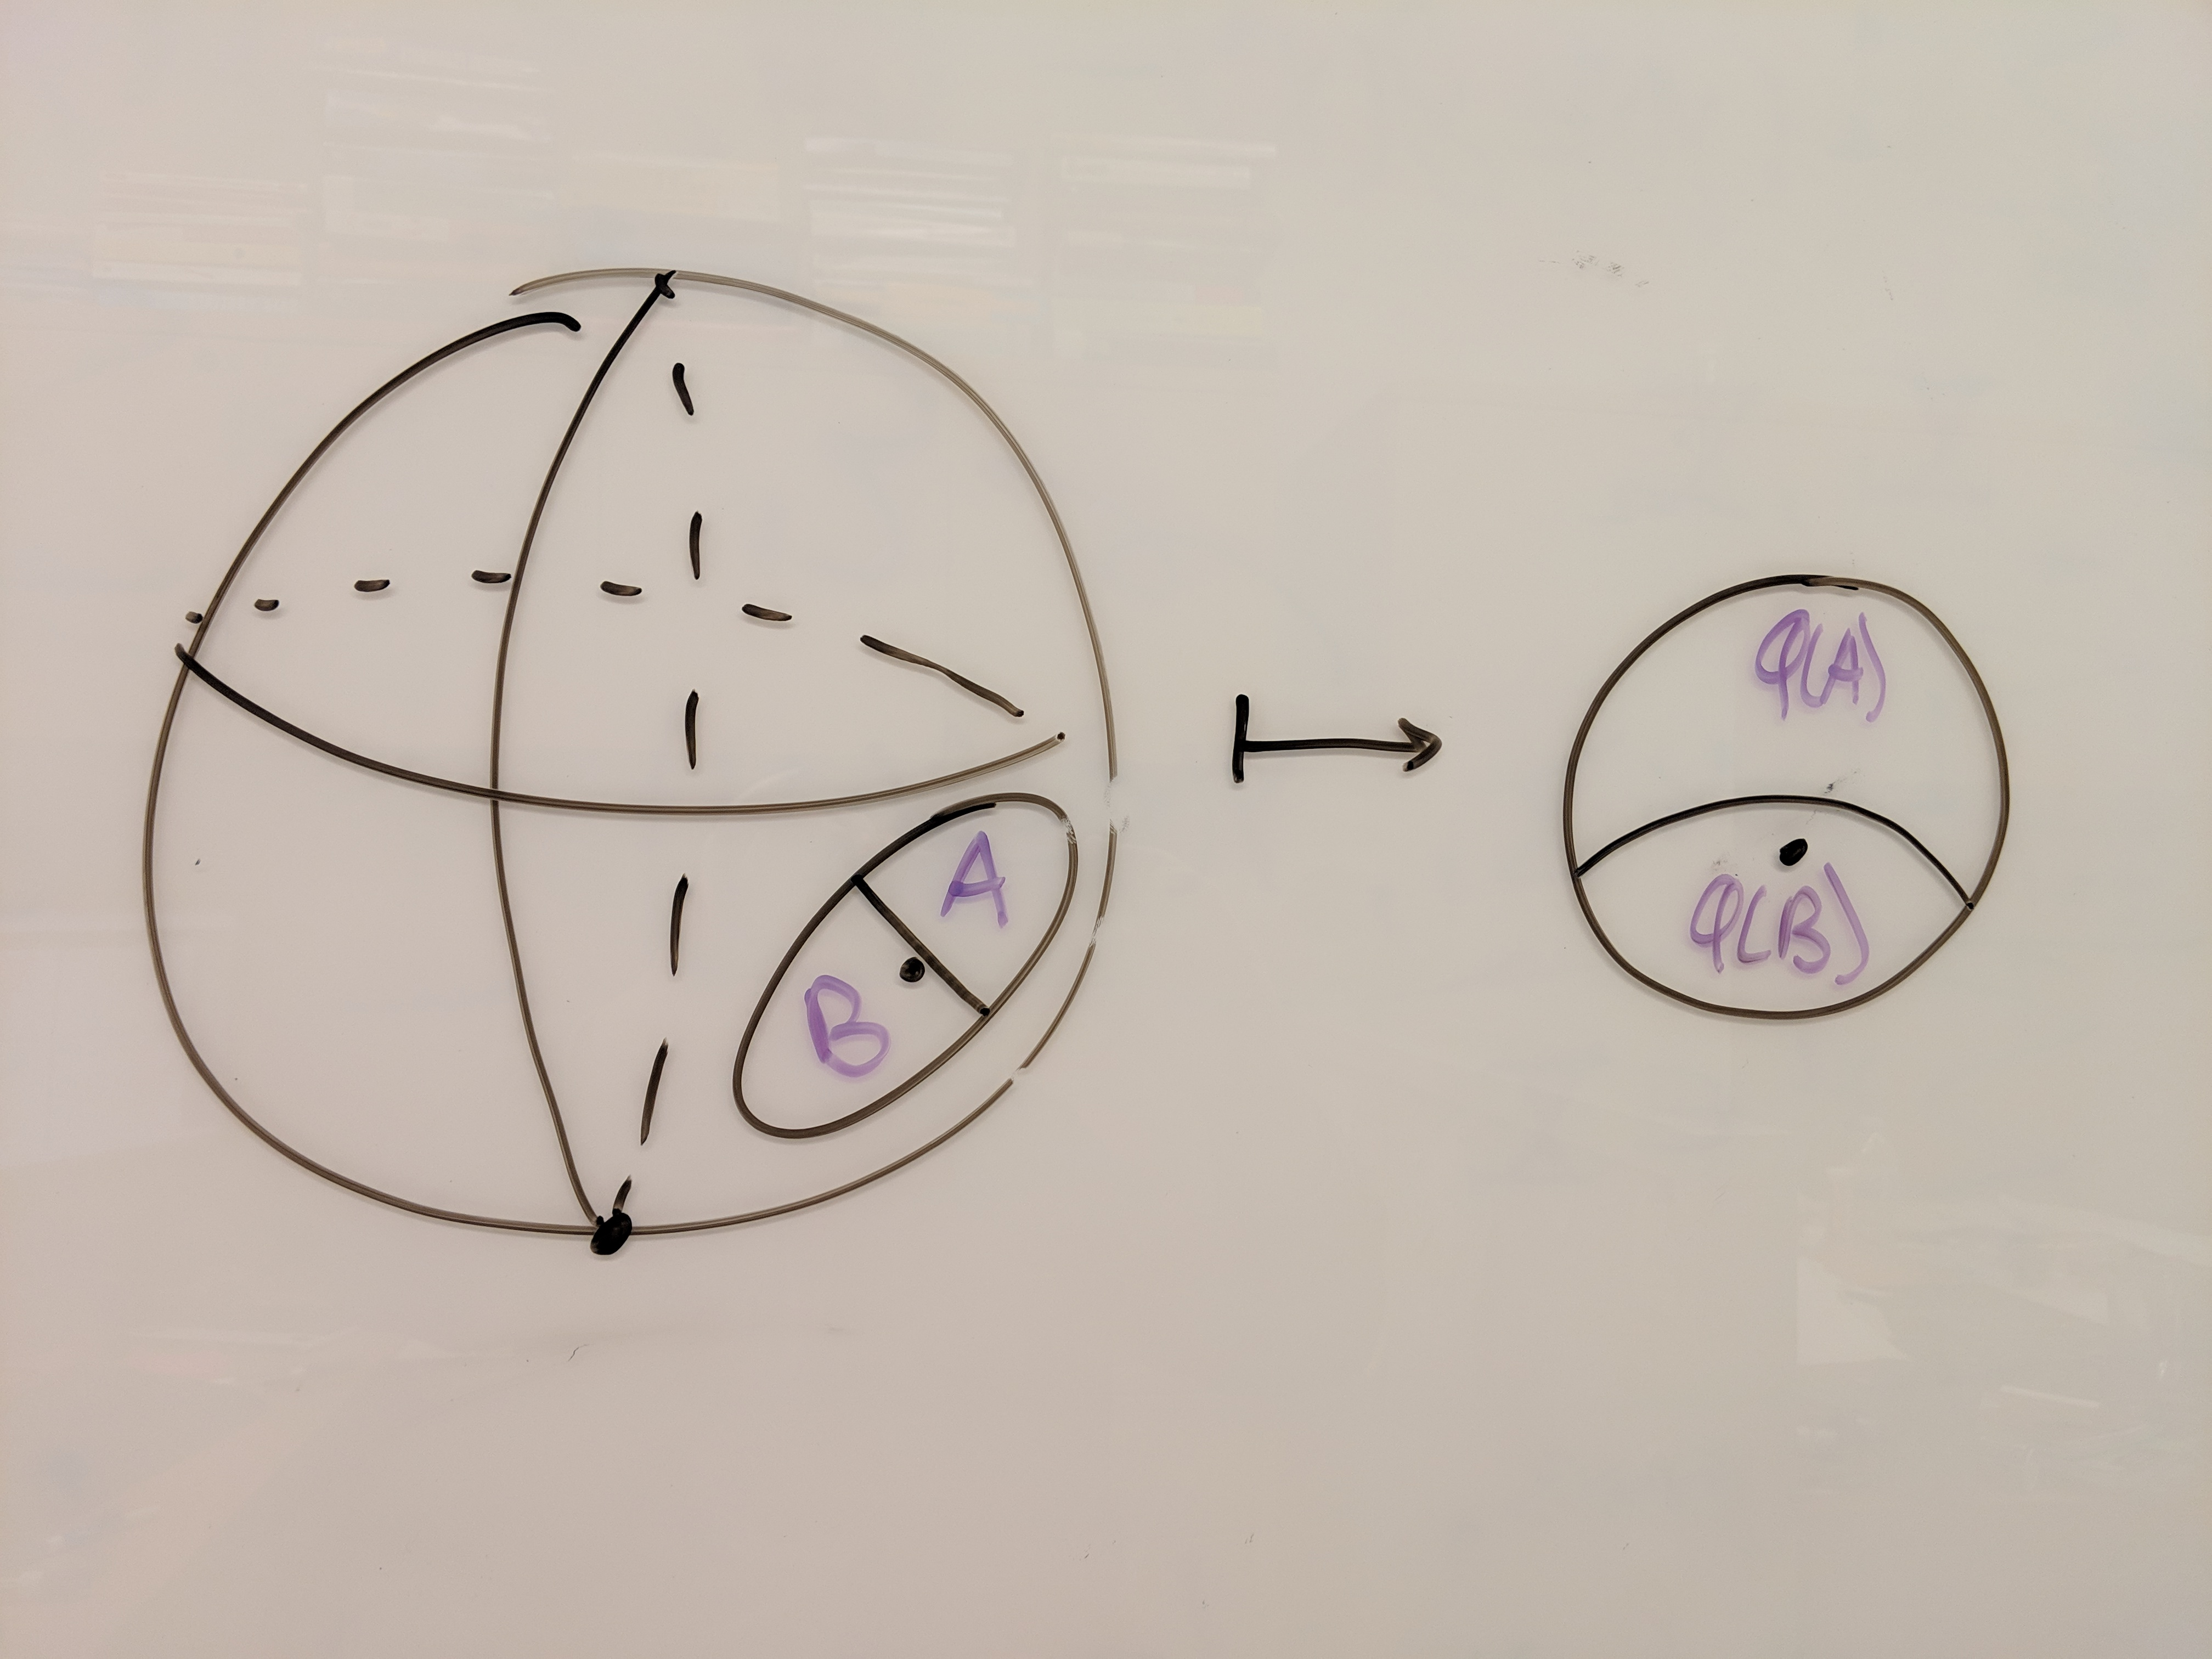
\includegraphics[width=.8\textwidth]{figs/stereo_ipq.jpg}\\
    \caption{ The image of a cap away from the south pole under the stereographic projection. }
    \label{fig:stereoipq}
\end{figure}



\begin{proof}
Using the same construction as in the proof of Theorem~\ref{thm:reock}, since the image under the stereographic projection of $\kappa'_N$ has both smaller area and larger perimeter than the image of $\kappa'_S$, the isoperimetric quotient score of the image of $\kappa'_N$ in the plane is strictly worse than the score of the image of $\kappa'_S$, although they have the same score as regions on the surface of the sphere.

\end{proof}


The remainder of the argument also follows from our previous results.  Lemma~\ref{lem:noafflin} says that no scaled isometry can correct for the permutation of score ordering, so there does not exist a map projection which preserves the ordering over regions induced by the isoperimetric quotient score.






